\chapter{\ifproject%
\ifenglish Project Structure and Methodology\else โครงสร้างและขั้นตอนการทำงาน\fi
\else%
\ifenglish Project Structure\else โครงสร้างของโครงงาน\fi
\fi
}

ในบทนี้จะกล่าวถึงหลักการ และการออกแบบระบบไปจนถึงขั้นตอนการออกแบบจากความต้องการของผู้ใช้งาน

\makeatletter

% \renewcommand\section{\@startsection {section}{1}{\z@}%
%                                    {13.5ex \@plus -1ex \@minus -.2ex}%
%                                    {2.3ex \@plus.2ex}%
%                                    {\normalfont\large\bfseries}}

\makeatother
%\vspace{2ex}
% \titleformat{\section}{\normalfont\bfseries}{\thesection}{1em}{}
% \titlespacing*{\section}{0pt}{10ex}{0pt}

\section{การติดต่อและคุยงานเพื่อสรุปความต้องการของสำนักทะเบียน}

% \begin{figure}
% \begin{center}
% % \includegraphics{800px-Briny_Beach.jpg}
% \end{center}
% % \caption[Poem]{The Walrus and the Carpenter}
% \label{fig:walrus}
% \end{figure}

\section{เงื่อนไขของการวางร่างปฏิทินการศึกษา}
  เนื่องจากจุดประสงค์ของโครงงานนี้คือต้องการพัฒนาเว็บไซต์ให้แก่สำนักทะเบียน
  จึงจะต้องเริ่มจากการพูดคุยกับบุคลากรของสำนักทะเบียนเพื่อให้ได้
  ความต้องการที่แก้จริงของโครงงานโดยในปฏิทินจะมีเงื่อนไขต่างๆ อันสรุปได้ดังนี้

\subsection{ภาคการศึกษาที่ 1}
  คาบเรียนของแต่ละวัน มีจำนวนดังนี้ วันจันทร์อย่างน้อย 14 คาบ วันอังคารอย่างน้อย 14 คาบ วันพุธอ่างน้อย 14 คาบ วันพฤหัสบดี 13 คาบ วันศุกร์ 12 คาบ(ประมาณ) \\
  - วันเปิดภาคเรียนมักจะเริ่มเดือนมิถุนายน \\
  - รูปแบบวันจันทร์ พฤหัสบดี มีระยะเวลาการเรียนการสอนตลอดภาคการศึกษา จำนวน 42 ชั่วโมง \\
  - รูปแบบวันอังคาร ศุกร์ มีระยะเวลาการเรียนการสอนตลอดภาคการศึกษา จำนวน 40 ชั่วโมง 30 นาที \\
  - วันลงทะเบียนเรียนล่วงหน้า สัปดาห์แรกของเดือนก่อนหน้าที่จะเปิดภาคการศึกษา \\
  - ประกาศผลการลงทะเบียนเรียนล่วงหน้าหลังจากลงทะเบียนล่วงหน้าประมาณ10วัน \\
  - วันลงทะเบียนเรียนมักจะเริ่มก่อนวันเปิดภาคเรียนวันแรก 1-2 วัน \\
  - วันลงทะเบียนมีระยะเวลา8วัน (เป็นเวลาที่ตรงกับวันเรียนด้วย) \\
  - วันถอนกระบวนวิชาโดยไม่ได้รับอักษรลำดับขั้น W จะเริ่มจากวันลงทะเบียนเรียน ถึงวันที่1ของเดอนถัดไป \\
  - วันที่อาจารย์ที่ปรึกษาให้ความเห็นชอบการลงทะเบียนเรียนของนักศึกษาทางระบบ Internet ระยะเวลาเริ่มจาก1สัปดาห์หลังจากเปิดภาคเรียนจนถึงวันที่1ของเดือนถัดไป \\
  - หลังจากหมดวันถอนกระบวนวิชาโดยไม่ได้รับอักษรลำดับขั้น W จะเริ่มนับวันถอนกระบวนวิชาโดยได้รับอักษรลำดับขั้น W \\
  - หลังจากเปิดภาคเรียน เมื่อเรียนครบ 8สัปดาห์จะเริ่มสอบกลางภาค \\
  - สอบกลางภาคสัปดาห์ที่9ของภาคเรียน มีระยะเวลาทั้งหมด7วัน \\
  - หลังจากวันสุดท้ายของการสอบกลางภาค เริ่มเรียนครึ่งภาคเรียนหลัง(สัปดาห์ที่10) \\
  - ครึ่งภาคเรียนหลังเวลาเรียนจะมีระยะเวลา7สัปดาห์ เริ่มสอบกลางภาค \\
  - วันสอบปลายภาคมีระยะเวลา2อาทิตย์ \\
  - หลังสอบปลายภาคจะทำการหยุดเรียนจนจบสัปดาห์นั้นและหยุดเรียนเพิ่มอีก 1สัปดาห์ และเปิดภาคเรียนที่2วนวันจันทร์ของสัปดาห์ถัดมา \\
\subsection{ภาคการศึกษาที่ 2}
  คาบเรียนของแต่ละวัน มีจำนวนดังนี้ วันจันทร์ 12 คาบ วันอังคาร 15 คาบ วันพุธ 15 คาบ วันพฤหัสบดี 15 คาบ วันศุกร์ 14 คาบ \\
  - รูปแบบวันจันทร์ พฤหัสบดี มีระยะเวลาการเรียนการสอนตลอดภาคการศึกษา จำนวน 40 ชั่วโมง 30 นาที \\
  - รูปแบบวันอังคาร ศุกร์ มีระยะเวลาการเรียนการสอนตลอดภาคการศึกษา จำนวน 43 ชั่วโมง 30 นาที \\
  - วันลงทะเบียนเรียนล่วงหน้า ก่อนเปิดภาคเรียน25วัน \\
  - ประกาศผลการลงทะเบียนล่วงหน้า1สัปดาห์ \\
  - เปิดภาคการศึกษาที่2(ระยะเวลา18 สัปดาห์เหมือนภาคการศึกษาที่1) \\
  - วันลงทะเบียนเรียนมักจะเริ่มก่อนวันเปิดภาคเรียนวันแรก 1-2 วัน \\
  - วันลงทะเบียนมีระยะเวลา8วัน (เป็นเวลาที่ตรงกับวันเรียนด้วย) \\
  - หลังจากสอบปลายภาคภาคเรียนที่2 จะหยุดเรียน3 สัปดาห์ \\
  - หลังจากหยุดเรียน3สัปดาห์ จะเริ่มเปิดภาคเรียนฤดูร้อน \\
\subsection{ภาคการศึกษาฤดูร้อน}
  ภาคฤดูร้อน มีรูปแบบการเรียนการสอน ตั้งแต่ วันจันทร์-วันศุกร์ ระยะเวลาที่ใช้สำหรับการเรียนการสอนแต่ละกระบวนวิชามีเวลาเรียนจำนวน 29 คาบ เท่ากับ 43 ชั่วโมง 30 นาที \\
  - ลงทะเบียนล่วงหน้าของภาคฤดูร้อนเริ่มหลังจากปิดภาคเรียนที่2 1สัปดาห์(ระยะเวลา 4 วัน) \\
  - ประกาศผลการลงทะเบียนล่วงหน้าหลังจากปิดการลงทะเบียน2วัน \\
  - วันเพิ่ม-ถอนกระบวนวิชา/ลงทะเบียน สำหรับนักศึกษาทุกระดับ ก่อนวันเปิดภาคเรียน 1สัปดาห์ \\
  - ภาคฤดูร้อนระยะเวลาเรียน6สัปดาห์ \\
  - สัปดาห์ที่7ของภาคฤดูร้อนจะเป็นสอบปลายภาคฤดูร้อน \\
  - หลังจากสอบปลายภาคฤดูร้อนแล้วจะปิดปีการศึกษา \\
  -วันไห้ครู หยุดเรียน \\

หลังจากที่ได้เงื่อนไขทั้งหมดครบแล้ว จะนำเงื่อนไขเหล่านี้มาแยกออกจากระบบที่ตอบสนอง \\
และเพิ่มความสะดวกสบายของผู้ใช้

\section{การทำงานของโปแกรม}
จากการสรุปความต้องการของสำนักทะเบียนผ่านทางบุคลากรจึงสรุปออกมาเป็น User Flowหรือ
สิ่งที่แสดงเส้นทางของผู้ใช้แอพพลิเคชั่นได้ดังนี้
\begin{figure}[h]
\centering
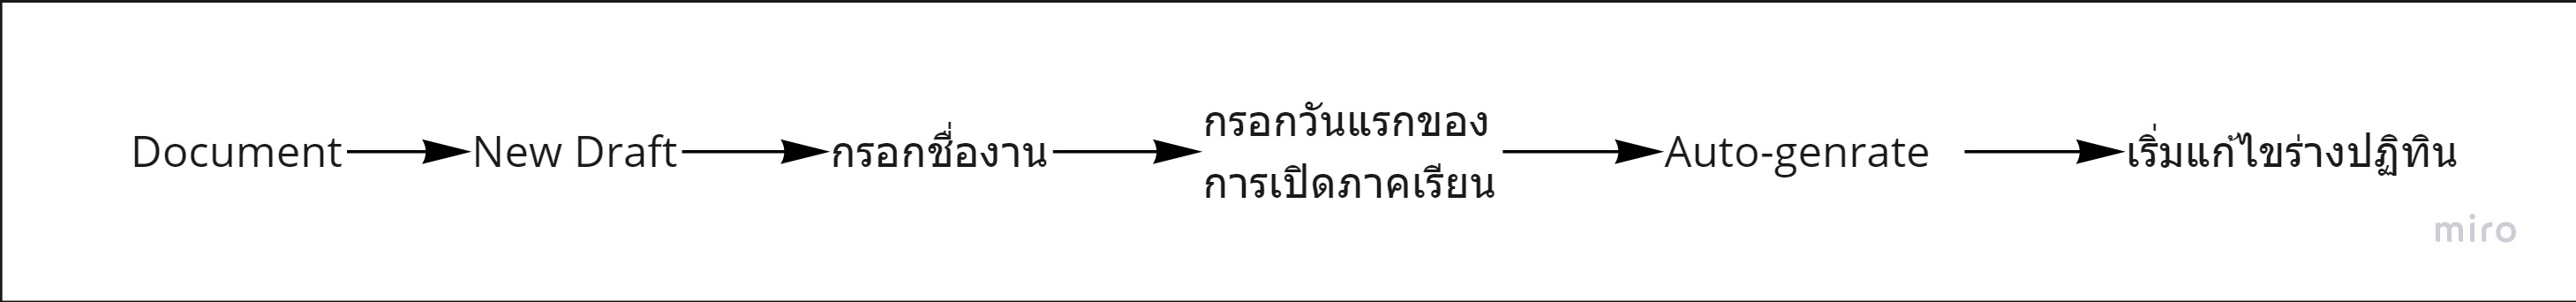
\includegraphics[width=1\textwidth]{pic3.1.jpg}
\caption{การทำงานเมื่อผู้ใช้ต้องการสร้างแบบปฏิทินใหม่}
\end{figure}
จากรูปที่3.1 ผู้ใช้จะเริ่มจากการเข้าสู่ระบบโดยใช้ CMU QAuthหลังจากนั้น คลิกที่สร้างดราฟใหม่ 
หลังจากนั้นเว็บไซต์จะต้องการทราบวันแรกของการเปิดภาคเรียนเพื่อนำไปสร้างปฏิทินการศึกษา
โดยหน้า Document จะเป็นหน้าที่ใช้จัดการกับร่างปฏิทินทั้งหมดที่ผู้ใช้ได้สร้างไว้
หลังจากที่ผู้ใช้ได้คลิกสร้างปฏิทินขึ้นมาใหม่ ระบบจะต้องการให้ผู้ใช้กรอกข้อมูลของวันเปิดเทอม
ของปีการศึกษานั้น หลังจากนั้นระบบจะทำการสร้างร่างปฏิทินการศึกษาแบบอัตโนมัติ
เพื่อทำให้ง่ายต่อการแก้ไข \\ ไม่เกิดความยุ่งยากในการต้องมาเพิ่มกิจกรรมทีละวันกิจกรรม
โดยกิจกรรมที่นำไปใส่ลงในปฏิทินแบบอัติโนมัตินั้นจะได้มาจากการคำนวน
วันที่อยู่ห่างจากวันเปิดเทอมตามเงื่อนไขของปฏิทิน
% วางรูป Dupilicate flow\
% รูปที่3.2 การทำงานเมื่อผู้ใช้ต้องการทำซ้ำปฏิทินเดิม

\section{โครงสร้างของโครงงาน}

\begin{figure}[h]
\centering
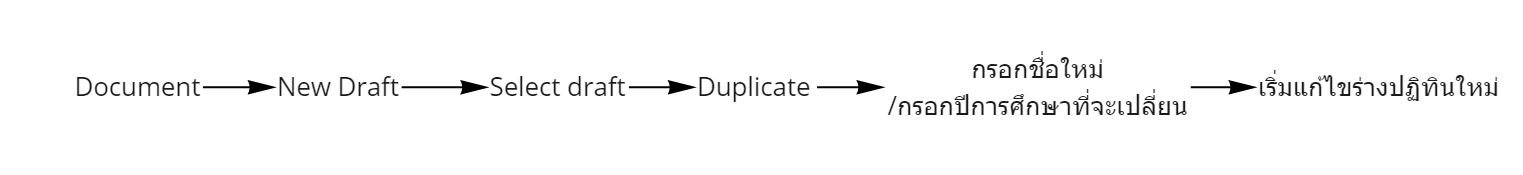
\includegraphics[width=1\textwidth]{pic3.2.jpg}
\caption{การทำงานเมื่อผู้ใช้ต้องการสร้างแบบปฏิทินใหม่}
\end{figure}

จากรูปที่3.2 ผู้ใช้ต้องการจะทำซ้ำ หลังจากที่ผู้ใช้อยู่ในหน้า Document และคลิกที่ทำซ้ำหรือ \\ Dupilicate
เว็บไซต์จะต้องการให้ผู้ใช้กรอกชื่อของปฏิทินที่จะสร้างใหม่ที่ทำซ้ำมาจากปฏิทินเดิม
และปีที่ต้องการเปลี่ยนใหม่ หากมีกิจกรรมของปฏิทินเดิมที่คล้ายคลึงกับปฏิทินของปีถัดไป 
ผู้ใช้สามารถทำซ้ำปฏิทินเดิมแล้วเปลี่ยนเป็นปีถัดไปได้เลย

\section{โครงสร้างโปรแกรม}
ในส่วนของ Client จะใช้ภาษา React.JS ในการสร้างเว็บไซต์ แพลตฟอร์มนี้จะใช้กับ
คอมพิวเตอร์ โดยมี Node.JS ในส่วน Backend และใช้ API ในการรับส่งกับฐานข้อมูล
และฐานข้อมูล MongoDB